
\chapter{Cluster Uandes}
\label{uandes_cluster}

Parte del inicial desarrollo de la presente memoria consistió en construir junto a un equipo de trabajo de la Universidad De los Andes un cluster de super-cómputo nocturno dentro de la casa de estudios. Dicho cluster fue elaborado con el objetivo de utilizar los recursos de la universidad y experimentar con las diferentes técnicas propuestas la existencia o no de una mejora frente a dichos esquemas de particionamiento. Para el desarrollo del super-computador, se utilizaron 30 de los ordenadores con los que la universidad cuenta en el laboratorio de \textbf{FICA}. El equipo de trabajo espera integrar más nodos en el futuro.

\begin{figure}[H]
\begin{center}
   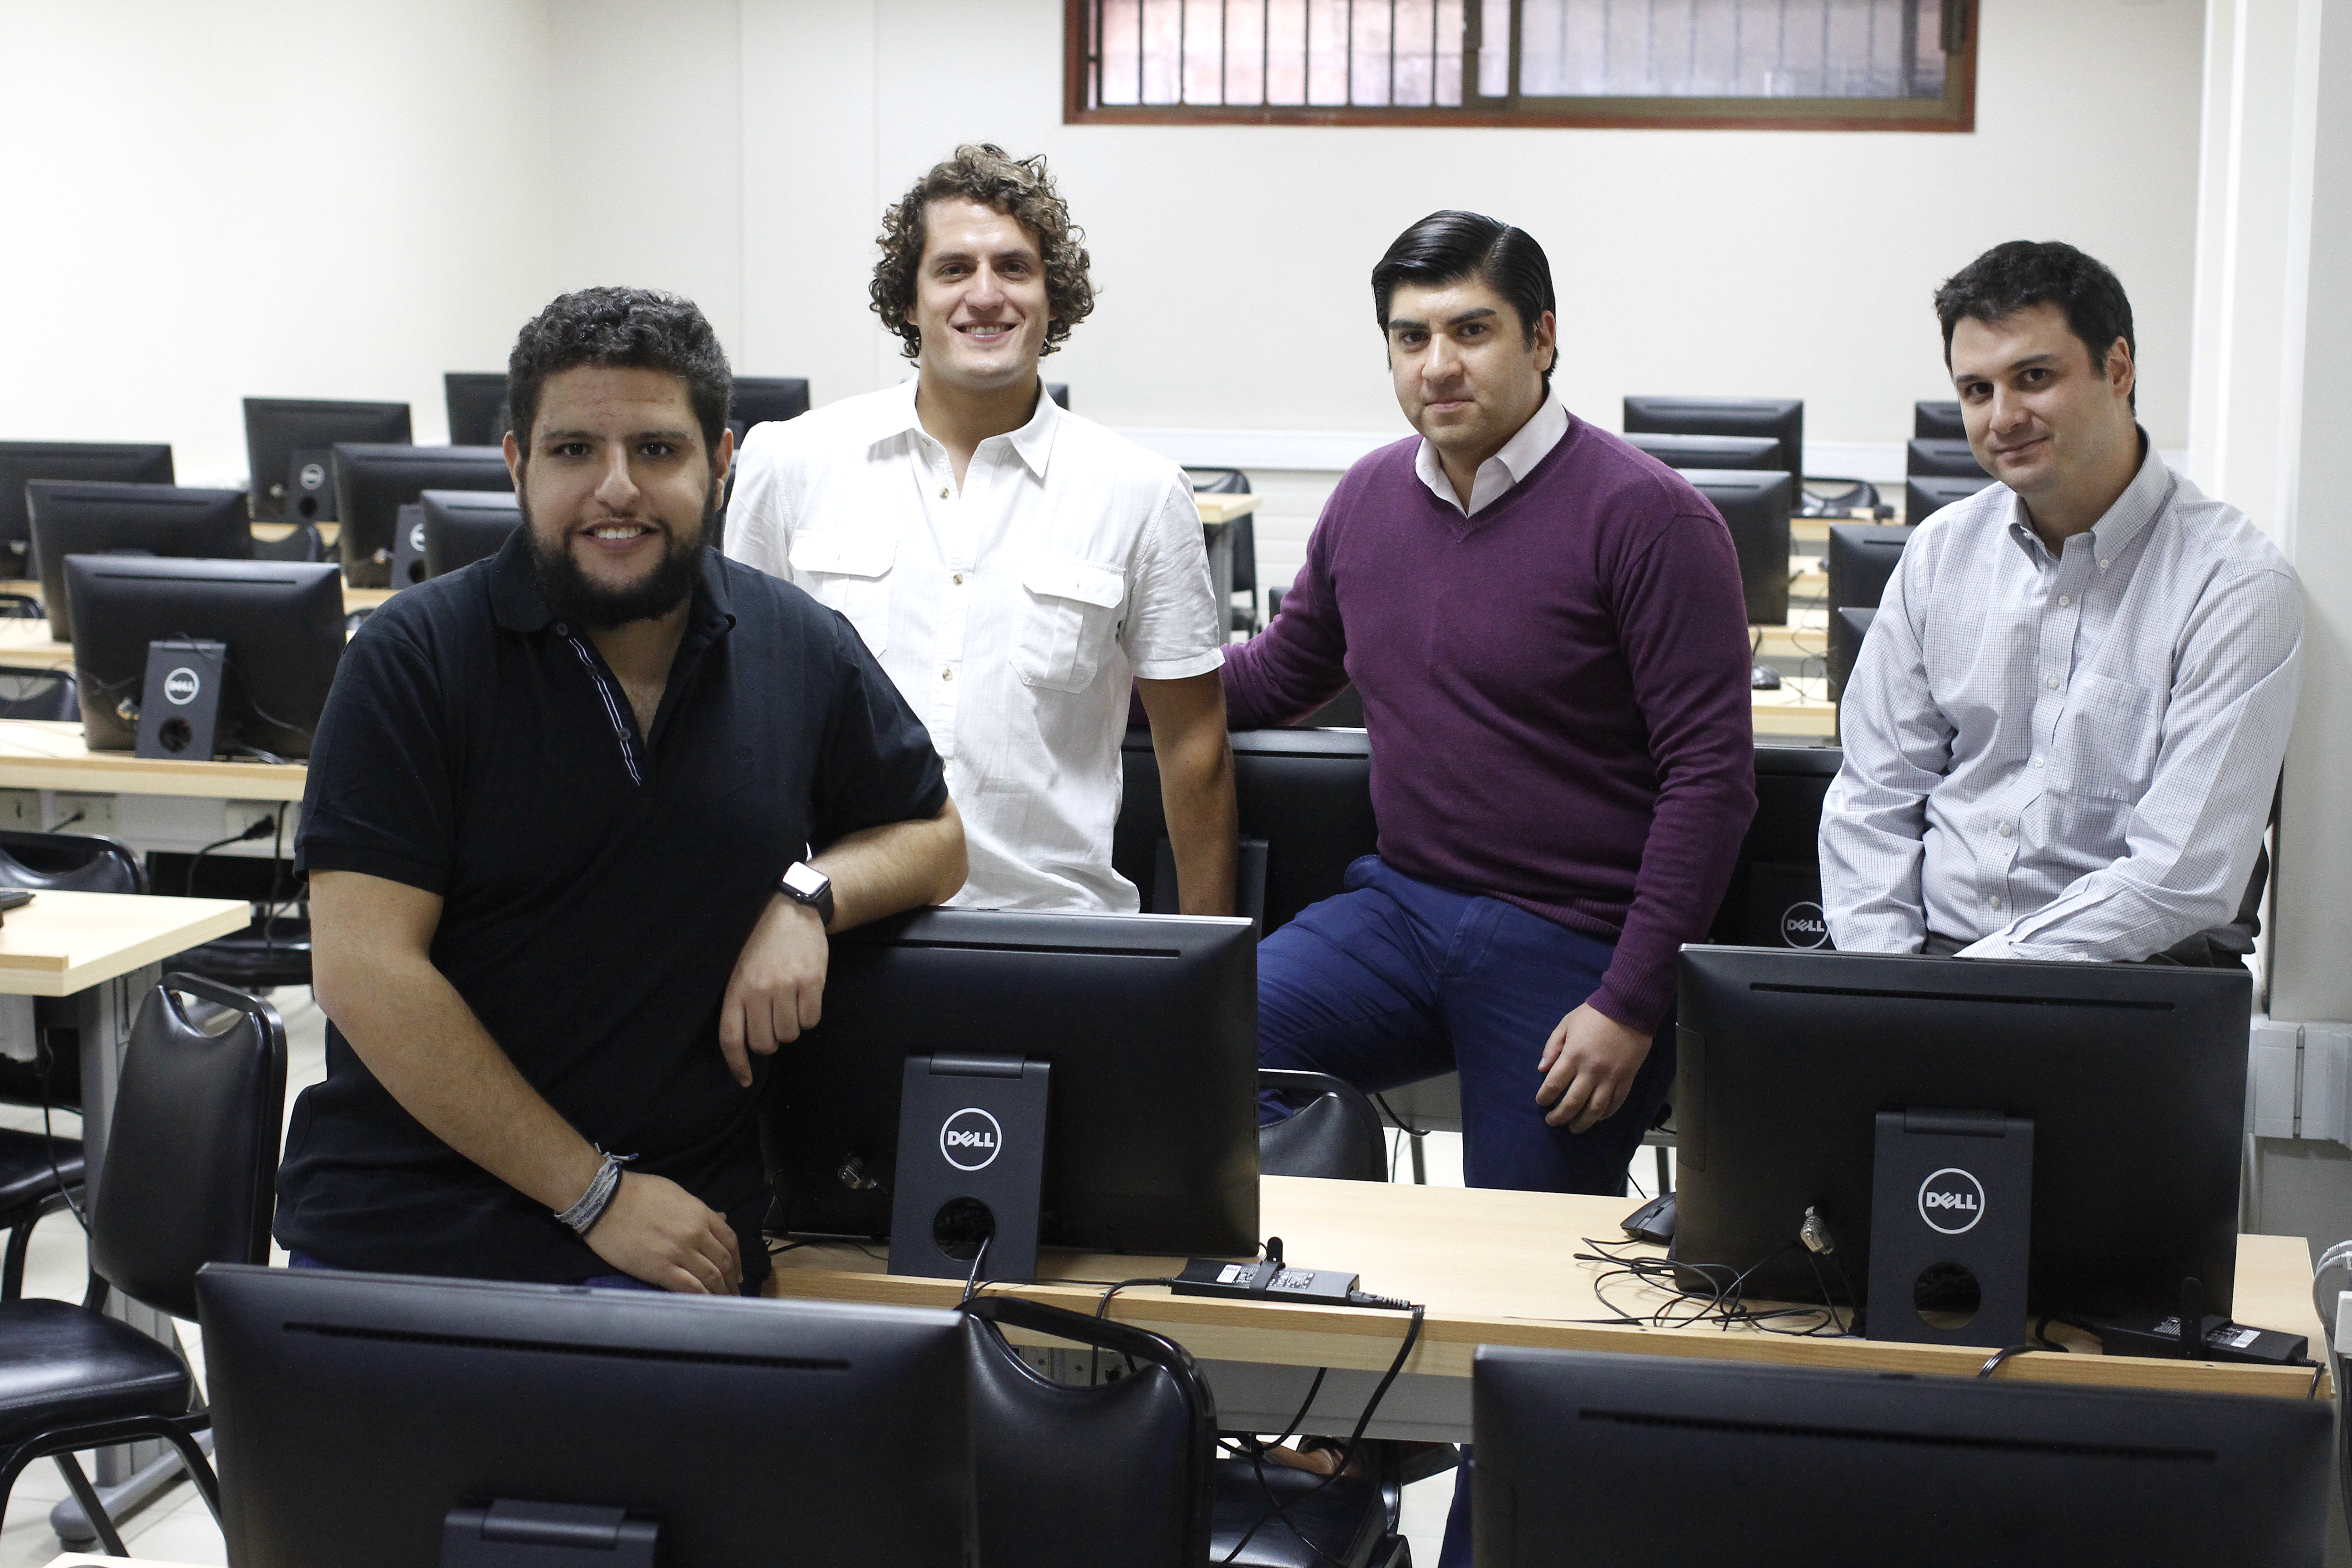
\includegraphics[scale=0.083]{images/c03/Supercomputador2.JPG}
\end{center}

%texto que aparece al pie de la figura
\caption[Equipo de trabajo Cluster Uandes]{Equipo de trabajo Cluster Uandes (Universidad de los Andes)\footnotemark{}. El equipo elaboró planificó y elaboro el cluster el primer semestre de 2018 y espera terminar las configuraciones finales en septiembre de 2018.}
\label{c03_cluster_uandes_team} % etiqueta para ser usada por referencias desde el texto
\end{figure}
\footnotetext{Fuente: \url{http://www.uandes.cl/noticias/ingenieros-uandes-desarrollan-supercomputador-nocturno-en-laboratorio-de-la-facultad.html}}

A diferencia de Leftraru, el cluster Uandes se elaboró con componentes que no están diseñados para HPC. Por un lado, los nodos de cómputo son computadores de escritorio donde el uso esperado es la ejecución de programas para el alumnado de la Universidad. Al mismo tiempo, la red de trabajo es \textit{ethernet} por medio de un switch convencional. Esta red de trabajo es apropiada para el uso cotidiano dentro de la universidad, pero es extremadamente limitada a la hora de ejecutar aplicaciones de HPC tanto por la latencia como por el ancho de banda que puede proveer, siendo incapaz de sostener el uso intensivo que ciertas aplicaciones de HPC como OpenSees requieren. Al igual que Leftraru, el cluster fue configurado para poder correrse bajo diferentes configuraciones y números de núcleos.


\begin{figure}[H]
\begin{center}
   \includegraphics[scale=0.145]{images/c03/cluster_uandes.jpg}
\end{center}

%texto que aparece al pie de la figura
\caption[Cluster Uandes en ejecución]{El Cluster Uandes fue elaborado con el apoyo de la propia Universidad y la facultad de Ingeniería y Ciencias Aplicadas con el objetivo de experimentar con ambientes distribuidos y hacer un uso más efectivo de los recursos de la Casa de estudios. Se pretende que la unidad quede operativa para quedar disponible de manera nocturna frente a las necesidades de los investigadores de la Universidad por medio de una cola de trabajo implementada por Slurm.}
\label{c03_cluster_uandes} % etiqueta para ser usada por referencias desde el texto
\end{figure}

El cluster Uandes posee las especificaciones de la Tabla \ref{table_uandes_cluster_configuration}.

\begin{table}[H]
\begin{tabular}{p{5cm}p{9.3cm}} \toprule
    \textbf{Componente} & \textbf{Descripción}\\ \midrule
    Nombre Cluster & Uandes \\
    Nodos de cómputo & 30 nodos de cómputo Desktop Dell 3050 AIO Series\\
    Cantidad de cores & 120 \\
    Co-Procesadores & No \\
    RAM & 480 GB de RAM \\
    Conexión & Ethernet\\
    Almacenamiento & N/A\\
    Capacidad de cómputo & N/A \\
    \bottomrule

\end{tabular}
\caption[Especificaciones cluster Uandes]{Especificaciones cluster Uandes}
    \label{table_uandes_cluster_configuration}
\end{table}

Se espera que durante el segundo semestre de 2018, las simulaciones ejecutadas en el cluster Leftraru sean replicadas en el super-computador Uandes para determinar así cómo inciden los esquemas de particionamiento en la topología del cluster.
